\chapter{Data Preparation}
Verbleibend sind die unbereinigten Überschriften.
Außerdem ist bereits auffällig geworden, dass eine möglich Zielvariable im vorhanden Datensatz fehlt. Alle vorliegenden Daten sind bislang unbewertet. Im Sinne unserer Forschungsfrage gilt es im Schritt der Konstruktion der Daten die entsprechende Zielvariable zu evaluieren und zu ergänzen, um so eine geeignete Bewertung bzw. Gewichtung der Überschriften herleiten zu können.
Als Zielvariable erscheint der Aktienkurs geeignet. Dieser bietet ein objektives Abbild des Wertes der Aktie zum gegebenen Zeitpunkt. Somit verbleibt es dem Modell eine Verbindung zwischen der Veröffentlichten Headline und der Veränderung des Aktienkurses herzustellen.

\section*{Bereinigen}
Aufgrund der Beschränkungen durch die kostenfreie Version, der zugrunde Liegenden API, zur Ergänzung der Aktienpreise zu den entsprechenden Headlines, sind wir gezwungen den Datensatz auf die letzten Zwei Jahre zu verkürzen.
Dies hat kein semantischen Auswirkungen. Nicht abzustreiten, das entsprechende Modell würde ungemein genauer werden, wenn mehr historische Daten zur Verfügung stehen würden. Doch semantisch stellt die Anzahl der verwendeten Einträge und Insbesondere die Anzahl der verwendeten Stocks keinen Einflussfaktor dar, es werden keine möglichen Predictoren entfernt. Auf der anderen Seite allerdings ist es durchaus möglich dass das Modell, aufgrund des starken und schnellen Wandels des Aktienmarktes, eine zeitlich begrenzte Gültigkeit besitzt. \\
Denkbar ist eine Gewichtung des Einflusses von Headlines auf Aktien, welche nur sehr wenig oder sehr oft, über einen längeren Zeitraum, erwähnt werden. Dies ist sicherlich ein Interessantes Forschungsthema, jedoch nicht Teil dieser Arbeit.\\
Da nur 4\% der Daten Uhrzeiten beinhalten, werden die Zeitstempel auf Tage reduziert. Somit ist nur eine tagesgenaue vorhersage möglich.
Nach der Bereinigung der Daten besteht der Datensatz nun mehr aus rund 164698 Einträgen mit einer Zeitspanne vom 21.August 2019 bis zum 11.Juni 2021.\\

\section*{Konstruieren}
Wie einleitend schon erwähnt gilt es nun die Zielvariable zu ergänzen. Hierfür nutzen wir eine API die zu den jeweiligen Aktienkennungen (Ticker) die entsprechenden Aktienpreise liefert. Bei Angabe des Tickers, eines Zeitraumes und eines Intervalls, erhält man jeweils die Börsenpreise zu Börsenbeginn (open), Börsenschluss (close), den Maximalpreis (high) und den Tiefspreis (low) zum entsprechenden Zeitpunkt. \\Verwendet wird ''Polygon.io''. Aufgrund der nur tagesgenauen Daten verwenden wir für jede eindeutige Aktie, nach oben beschriebenen Kriterien, ein Intervall von einem Tag innerhalb der letzten Zwei Jahre zwischen dem 21.August 2019 und 31. Dezember 2020. Die jeweiligen Aktienpreise werden dann zum Datensatz ergänzt. Hier gilt es ein entsprechendes Intervall vor und nach Veröffentlichung heranzuziehen, die Größe des Intervalls wird später erörtert. Überschriften, zu denen die API keine Aktienpreise nennen kann werden aus dem Datensatz entfernt. Meist sind solche Überschriften zu den Schließzeiten der Börse erschienen, um die Auswirkungen der Headline jedoch entsprechend zuordnen zu können, werden diese Einträge nicht weiter betrachtet. \\
Nach dem grundsätzlichem Bereinigen des Datensatzes muss nun jede einzelne Überschrift bestimmten Schritten unterzogen werden, die später für das Modelling benötigt werden, im folgenden Headline Cleaning bezeichnet. Für das Preprocessing einer Headline greifen wir auf übliche Methoden zurück, und orientieren uns im folgenden an den Algorithmen angelehnt an \cite{agarwel2016}\\ 

\fbox{\begin{minipage}[t]{\linewidth}
Algorithmus 1: Preprocessing jedes Wortes
\begin{enumerate}
    \item Einzelne Headline eingeben
    \item Headline mit POS-Tagger taggen
    \item Lemmatisierung jedes Wortes
    \item Ausgeben jedes Wortes als Input für eine weitergehnde Unteruschung mit SentiWordNet
\end{enumerate}
\label{algo1}
\end{minipage}}%

\fbox{\begin{minipage}[t]{\linewidth}
Algorithmus 2: Analyse einer Headline
\begin{enumerate}
    \item Alle Headlines H der Nachrichten identifizieren
    \item Jede einzelne Headline mit dem Algorithmus 1 \ref{algo1} für SentiWordNet Analyse vorbereiten
    \item Für jedes Wort jeder Headline mit SentiWordNet einen Sentiment Score berechnen (score = postiv - negativ)
    \item Falls score < 0, setzte Sentiment auf -1
    \item falls score > 0, setze Sentiment auf +1
    \item sonst: setze score = 0
\end{enumerate}
\end{minipage}}

Die im Algorithmus 1 präsentierten Schritte ergänzen wir im Folgenden um kleinere, aber sehr häufig durchgeführte Normalisierungsschritte. Grundsätzlich werden aber folgende Schritte durchgeführt: Tokenization, Part-Of-Speech Tagging (im Folgenden POST), Stopword Removal und Lemmatization sowie Stemming. Die Tokenization spaltet einen Satz in einzelne Worteinheiten (die Tokenz) auf. Wir verwenden standardmäßig immer an Leerzeichen, sodass ein Token meisten ein einzlens Wort ist. Die Tokenization ist notwendig, um in den nächsten Schritten jedes einzelne Wort betrachten zu können. POST ist ein Verfahren zur Vorbereitung eines Opinion Mining (auch häufig Sentiment Analyse genannt). Mit POST kann analysiert werden, welcher Wortart ein Wort zugehörig ist. Dabei unterscheiden wir zwischen Nomen, Adjektiven, Adverben und Verben. Durch das explizite POST kann die sich anschließende Lemmatisierung der Wörter effizienter und genauer durchgeführt werden. Im weiteren werden Stopwords entfernt, die anährend keine Bedeutung für den Bedeutung einer Aussage (in unserem Fall einer Headline) haben. Dazu gehören unter anderem Wörter wie "that", "is", "a". Daran anschlißend führen wir eine Lemmatization durch. Jedes Wort wird damit in seine Wörterbuchform überführt.
\\
Im ersten Schritt, vor der Tokenization, konvertieren wir nun also alle Wörter zur Vereinheitlichung in Kleinbuchstaben. Anschließend führen wir eine Tokenization durch. Dafür wird die im NLTK Modul enthaltene und von den Entwickler:innen des Moduls empfohlene Funktion word\_tokenize verwendet. In \cite{agarwel2016} wird ein POS-Tagger mit einer Accuracy von 97.24\% verwendet. Aus Gründen der Einheitlichkeit und der Zielsetzung verzichten wir an dieses Stelle darauf, diesen POS Tagger einzubinden, sondern nutzen den im NLTK Package enthaltenen und von dessen Entwickler:innen empfohlenen POS Tagger. In Abbildung \ref{Zwischenergebis_1} ist ein Ausschnitt des Zwischenergebnisses des Data Cleanings zu sehen.
\begin{figure}[t]
    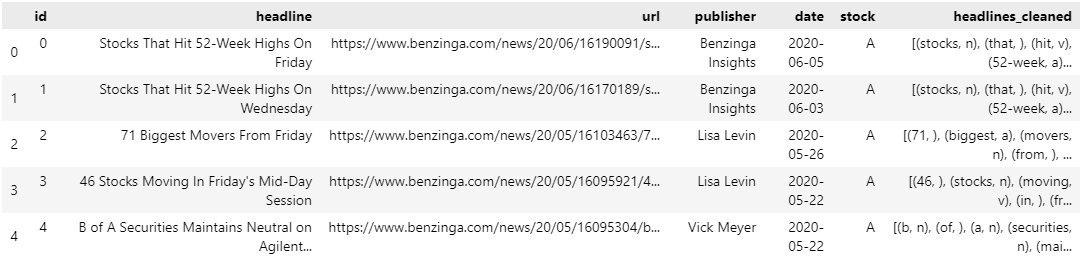
\includegraphics[scale=0.54]{img/Ausschnitt_Zwischenergebnis.png}
    \caption{Zwischenergebnis nach Tokenization, POST und Kleinschreibung}
    \label{Zwischenergebis_1}
\end{figure}
\\
Im nächsten Schritt werden die Stopwords entfernt. Auf diesen Schritt folgt nun die Lemmatizierung mittels dem Wordnet Lemmatizer. Wordnet ist ein lexikalisch-semantisches Netz, das seit 1985 an der Princteon University entwicklet wird. Es verfügt über zusammenhänge zwsichen Wörtern  \citep{miller1995}, und ist die Grundlage für viele andere Lexika, wie bspw. SentiWordNet \citep{bacianella2010}. Durch das POST weiss die Lemmatizer Funktion, um welche Wortart es sich handelt, und kann demetsprechend das jeweilige Wort auf die jeweilige Wörterbuchform zurückführen. Zu Vereinfachung behandeln wir alle Wörter, die beim POST keiner Wortart zugeordnet werden konnten, wie Nomen. Dahinter steht die Überlegung, keine Wörter zu verlieren, die im späteren Verlauf durch das SentiWordNet mit einem Senitment belegt werden könnten. Wir entfernen anschließend erneut weitere Wörter, nämlich jene, die weniger als drei Buchstaben haben sowie solche, die aus Zahlen bestehen, also numerisch sind.\\
\begin{figure}[t]
    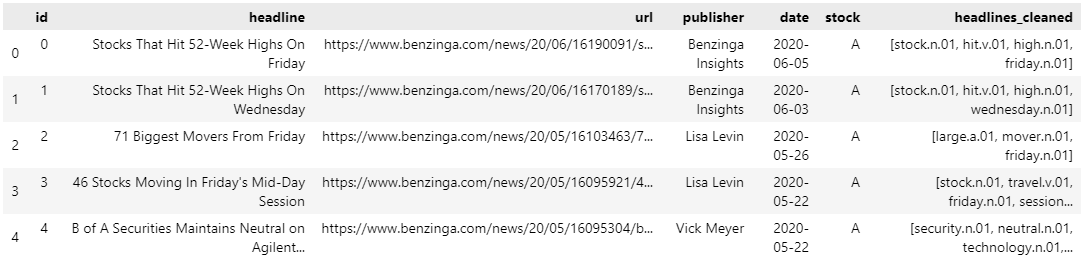
\includegraphics[scale=0.54]{img/Ausschnitt_Zwischenergebnis_2.png}
    \caption{Zwischenergebnis Snyset Format}
    \label{Zwischenergebnis_2}
\end{figure}
Mithilfe von SentiWordNet werden nun die Sentiments für jede Headline bestimmt. Dabei ergibt sich ein Senitment Score durch die Differenz zwischen poitivem Sentiment und negativem Sentiment. Diese Werte werden duch SentiWordNet geliefert und an die entsprechende Zeile ergänzt.

\section*{Integrieren}
Die bislang zwei Datensätze der Headlines mit dem Stockticker sowie dem SentimentScore und der Stockprices müssen, zur Verwendung im Modell, vereint werden. Dazu ergänzen wir jedem Eintrag des ersteren Datensatz mit dem \textit{open}-Kurswert und dem \textit{close}-Kurswert der jeweiligen Aktie am Tag der Veröffentlichung des Artikels. Um die Auswirkungen möglichst eindeutig zuweisen zu können, sollte ein entsprechend kleines Intervall verwendet werden. Um jedoch alle Auswirkungen zu erfassen, darf dieses auch nicht zu klein sein. Wir gehen davon aus, dass im Mittel, die Artikel nach Eröffnung des Aktienhandelsplatz und vor Schließung dessen publiziert werden. Dies ist auch auf der Webseite von Benzinga.com nach zu vollziehen. So wählen wir zu jeder Headline den Aktienkurs beim öffnen des Aktienhandelsplatz als Referenzwert und den Preis beim schließen als Zielvariable.  
%ToDo: discuss intervall of stockprices to headline publish
In dem nun vereinten Datensatz ergänzen wir zusätzlich noch, aus dem Datensatz berechenbare, Werte wie den \textit{Stockprice\_Change} und \textit{Senti\_Binary}. Die jeweiligen Werte des Stockprice\_Change bilden die Veränderung des Stockprices am Tag der Veröffentlichung der Headline vom Eröffnungskurs zum Kurs beim Schließen der Börse ab. Dabei nimmt die Spalte des Stockprice\_Change eine 1 an wenn sich der Wert der Aktie um mehr als 1\% steigert, -1 wenn die Aktie um mehr als 1\% fällt. Sonst eine 0, wir gehe davon aus, das die Aktie sich nicht Nennenswert geändert hat, bzw. die Headline als Ursache für die Veränderung des Aktienpreises ausgeschlossen werden kann. Die jeweiligen Werte des Senti\_Binary ergänzen den Datensatz um eine drei-tuple Betrachtung des Sentiment. Ist der verrechnete Sentiment, aus der Anzahl der Wörter mit Negativen und Positiven Sentiment, insgesamt positiv, also größer 0, so ist Senti\_Binary eine 1. Ist der Sentiment negativ, also kleiner 0, so ist der Senti\_Binary -1. Sonst 0.

\section*{Formatieren}
Wie bereits ausführlich beschrieben, wurde das Datumsformat auf yyyy-mm-dd reduziert. Weitere Formatierungen wurden nicht unternommen, die Daten verbleiben in der Form wie sie konstruiert wurden.

\section*{Ergebnis}
Der anfangs schon betrachtete Datensatz wurde nun um die bereinigten Überschriften, den Sentiment-Scores und den Aktienpreisen erweitert. Außerdem wurden die Einträge stark reduziert, unter anderem durch die Festlegung einer Datumsspanne zwischen dem 21.August 2019 und 31. Dezember 2020.\\ 
64456 headlines haben einen durchschnittlichen Sentiment von 0, davon haben 59718 weder einen positiven noch einen negativen Sentiment-Score. 
Hingegegen haben 97022 Headlines einen Sentiment-Score gesetzt der ungleich 0 ist. 45005 positive, 52017 negative. Dabei haben 50671 jeweils positive und negative zu bewertende Wörter.\\ \\
Es verbleiben 3722 Stocks und 76162 eindeutige Überschriften. Insgesamt also 14 Spalten auf 161478 Einträge.
Die folgende Abbildung bietet einen Überblick über den aktuellen Datensatz, welcher für das Modeling verwendet wird. Zu Übersichtszwecken wurden die Spalten \textit{url} und \textit{publisher} ausgeblendet.
\begin{figure}
    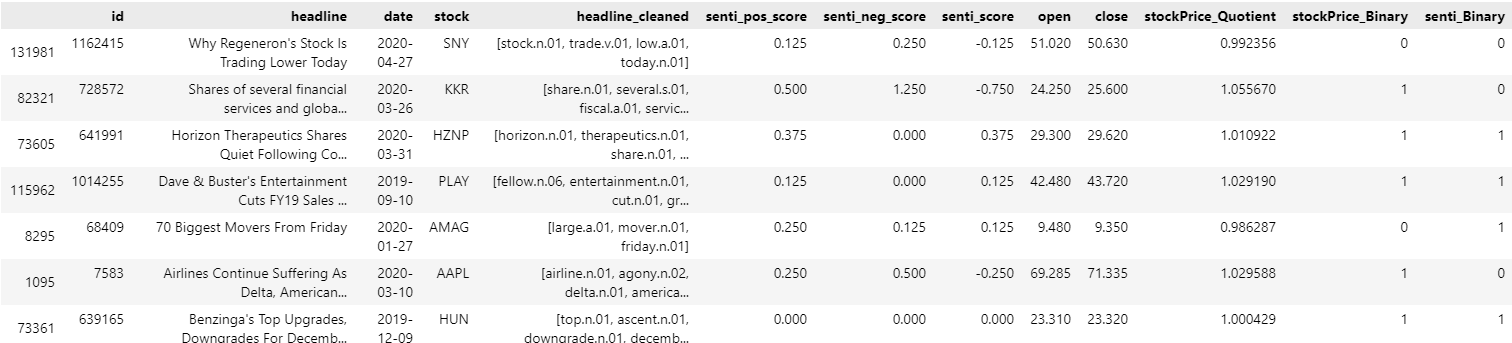
\includegraphics[width=1\textwidth]{img/dataSample7_constructed.png}
    \caption{Überblick über den konstruierten Datensatz, Sieben zufällige Einträge (url, publisher ausgeblendet)}
\end{figure} \\
Auch in den Überschriften selbst sieht man nach der Bereinigung einige Unterschiede. Ersichtlich ist, dass die Headlines vorrangig über die Lage des Handels berichten, so erscheinen Wörter wie ''Trade'' in Kombination mit ''high'' und ''low'' häufig. Jedoch erkennt man auch, dass einige Wörter wie ''company'', ohne weitere Aussagekraft, immer noch häufig verwendet werden. Vermutlich aufgrund des verwendeten, nicht spezifischen Stopword-Dictionary im Schritt des Stopword-Removal.
\begin{figure}
    \centering
    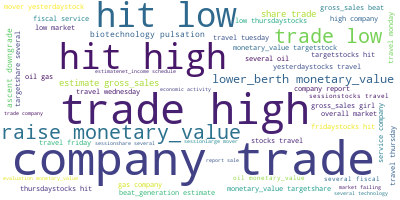
\includegraphics[scale=0.6]{img/wordcloud_afterCleaning.png}
    \caption{Top 50 Wörter im gesamten Datensatz, bereinigt}
\end{figure}